\documentclass[10pt,fleqn]{article} % Default font size and left-justified equations
\usepackage{import}
\usepackage[%
    pdftitle={SLCI : Transformée de Laplace},
    pdfauthor={Xavier Pessoles}]{hyperref}
\subimport{../../../../style/}{preambule.tex}
%\fichetrue
\fichefalse

\proftrue
%\proffalse

%\tdtrue
\tdfalse
\courstrue
%\coursfalse
\subimport{../../../../style/}{new_style}
\subimport{../../../../style/}{macros_SII}
\subimport{../../../../style/}{preambule_trou.tex}

\usepackage{siunitx}
\sisetup{inter-unit-product = \ensuremath { { } \cdot { } } }
% -------------------------------------
% Déclaration des titres
% -------------------------------------

\def\discipline{Enseignement \\Technologique \\ Transversal}
\def\xxtete{Enseignement Technologique Transversal}

\def\classe{1 STI2D}
\def\xxnumpartie{Séq 2}
\def\xxpartie{Modélisation des énergies au sein d'un système}

\def\xxnumchapitre{Séance 2}
\def\xxchapitre{\hspace{.12cm} Énergies, Puissances et rendement}

\def\xxposongletx{2}
\def\xxposonglettext{1.45}
\def\xxposonglety{23}
\def\xxonglet{Seq. 2 -- Se. 2}

\def\xxactivite{Cours}
\def\xxauteur{\textsl{Geoffrey Vaquette}}

\def\xxcompetences{%
\textsl{%
\textbf{Savoirs et compétences :}
\begin{itemize}[label=\ding{112},font=\color{ocre}]
\item CO2.1	Identifier les flux et la forme de l'énergie, caractériser ses transformations et/ou modulations et estimer l'efficacité globale d'un système.
\end{itemize}
%
}}

\def\xxfigures{
\begin{center}

\includegraphics[height=4cm]{images/smartphone.png} \\
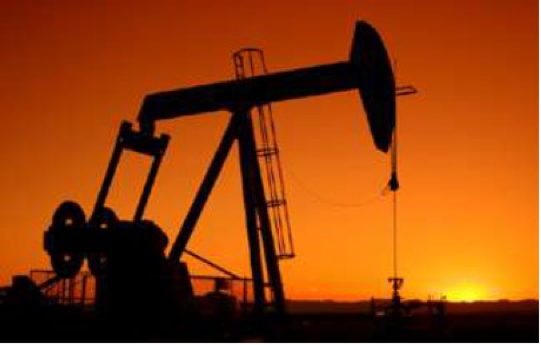
\includegraphics[width=0.7\textwidth]{images/petrole.png} \\
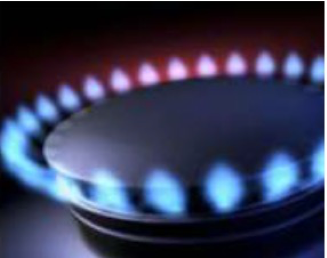
\includegraphics[width=0.7\textwidth]{images/gaz.png} \\
\end{center}
}%figues de la page de garde
\def\xxpied{%
Energies, Puissances et Rendement \xxactivite%
}

%---------------------------------------------------------------------------

\renewcommand{\RemplirTrou}{true}
\begin{document}
\chapterimage{png/Fond_solaire}
\subimport{../../../../style/}{new_pagegarde}


\section{Energie et puissance mécanique}
Une énergie mécanique est homogène à (partage les même unités que) une Force (en Newton N) multipliée par une longueur (en mètre m).
\subsection{Energie mécanique potentielle}
\begin{defi}
    Une masse \textbf{m} subissant une accélération \textbf{g} et pouvant réaliser un déplacement potentiel 
    \textbf{H} dispose d'une énergie potentielle 
    \trou{$E_p = P\times H,  E = m\times g\times H$, avec H en \si{m}, m en \si{kg} et g en \si{kg.m.s^{-2}}}. 
    Il s'agit de l'énergie que peut acquérir la masse lors de sa chute. 
\end{defi}


Sur terre, la gravitation vaut $g = 9.81 m.s^{-2}$

\begin{exemple}
    Un ascenseur, composé d'une cabine pesant \textbf{1000 kg} et accueillant 3 personnes pour une masse totale de \textbf{200 kg} se trouve au dernier étage, à une hauteur de \textbf{27m}. 
Quelle est l'énergie récupérable lors de la descente de l'ascenseur ? (En joule et en kWh) 

\afaire\trou{On calcule sa masse : $m = m1 + m2 = \SI{1200}{kg}$. On calcule l'énergie potentielle : $E_p = mgH = 1200 \times 9.81\times 27 = \SI{317,84}{J} $}

\correction \textbf{Correction : } \trou{On calcule sa masse : $m = m1 + m2 = 1200 kg$. On calcule l'énergie potentielle : $E_p = mgH = 1200 \times 9.81\times 27 = 317.84 J $}
\end{exemple}


\subsection{Énergie mécanique cinétique}
\subsubsection{Masse en translation}
\begin{defi}
  Une masse \textbf{m} se déplaçant dans un mouvement de \textbf{translation} à une vitesse \textbf{v} dispose d'une énergie cinétique \trou{$E_c = \frac{1}{2}m\times v^2$ avec m en kg et v en m/s}.   
\end{defi}

\begin{exemple}
    Une voiture de 1.5 tonne est lancée à 50 km/h. Calculez son énergie cinétique. 

\afaire \trou{On calule l'énergie cinétique : $E_c = \frac{1}{2} \times 1500 \times (50 000 \times 3600)^2 = 115 740 J = 115.7kJ $}

\correction\trou{On calule l'énergie cinétique : $E_c = \frac{1}{2} \times 1500 \times (50 000 \times 3600)^2 = 115 740 J = 115.7kJ $}
\end{exemple}


\subsubsection{Masse en rotation}
\begin{defi}
  Une \textbf{masse ponctuelle} \textbf{m} en rotation à une distance $l$ autour d'un axe $\Delta$ à la vitesse angulaire $\Omega$ dispose d'une énergie cinétique \trou{$E_c = \frac{1}{2} m \times l^2 \times \omega^2$}
\end{defi}


\subsection{Puissance mécanique : }
Puisque l'énergie mécanique est homogène à une force fois une longueur, la puissance mécanique est homogène à \trou{une force X une longueur / un temps (seconde) ou encore une force X une vitesse.}

\begin{defi}
  \paragraph{En translation : } Dans le cas de la translation, la puissance vaut : \trou{$P_{\text{meca}} = E/t = F\times L / t = F\times v$, en $W = Nms^-1$}
\paragraph{En rotation : }En rotation, la puissance mécanique peut se calculer comme le produit du couple $C$ par la fréquence de rotation $\Omega$. 
$P_{\text{meca}} = C \cdot \Omega$
\end{defi}

\pagebreak
\subsection{Energie et puissance électrique en courant continu}
\subsubsection{Energie électrique}
\begin{defi}
  L'énergie électrique se manifeste lors du déplacement de charges électriques (électrons ou ions). Ce déplacement est appelé \trou{courant électrique}, noté \trou{I} et exprimé en \trou{Ampère A}.

Une charge électrique (quantité d'électricité) se mesure en coulomb (C), \textbf{1 C correspond à un courant de 1 Ampère pendant 1 seconde.}
\end{defi}

\begin{defi}
  \paragraph{Energie électrique : } \trou{Une charge électrique $q$ soumise à une différence de potentiel $\Delta U$ dispose d'une énergie potentielle électrique $E_{elec} = q \Delta U$}
\end{defi}


\begin{exemple}
    

Un drône Parrot est équipé de 3 cellules au lithium délivrant chacune 334mA.h sous 11,1V. Déterminez l'énergie embarquée par ce drone en \textbf{kJ} puis en \textbf{W.h} lorsque la batterie est entièrement chargée. 

\afaire \trou{Calcul de la charge : $Q=334\times 10^{-3} \times 3600 = 1202.4 C$ On en déduit alors l'énergie : $E_{elec} = 3\times Q\times \Delta U = 40040 J = 11.1 Wh$}

\correction \trou{Calcul de la charge : $Q=334\times 10^{-3} \times 3600 = 1202.4 C$ On en déduit alors l'énergie : $E_{elec} = 3\times Q\times \Delta U = 40040 J = 11.1 Wh$}

\end{exemple}

\subsubsection{La puissance électrique d'un courant continu : }
La puissance électrique est le produit du courant \textbf{$I$} et de la différence de potentiel $\Delta U$, notée \textbf{$U$}. 

\begin{equation*}
    P = U\times I
\end{equation*}
\pagebreak
\section{La chaîne d'énergie}
Un système est une entité qui utilise de l'énergie afin d'\textbf{agir} sur une \textbf{matière d'oeuvre}. Le cheminement de l'énergie entre sa source et son utilsation concrète peut être modélisée par une succession de blocs appelée \textbf{Chaîne d'énergie}.

\begin{obj}
  Afin de décrire le fonctionnement d'un système, la chaîne d'énergie est un outil adapté faisant apparaître les différents organes impliqués dans l'adaptation et l'utilisation de l'énergie.
\end{obj}


\begin{center}
\vspace{0.3cm}
    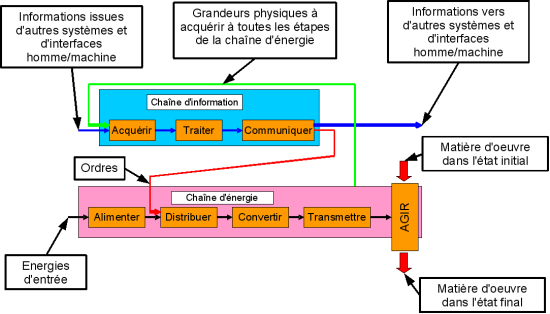
\includegraphics[width=0.8\textwidth]{images/Chainefonctionnelcomplete.png}
    \vspace{0.3cm}
\end{center}

\begin{defi}
La chaine d'énergie se décompose en différents blocs fonctionnels associés aux fonctions :

    \begin{description}
  \item[Alimenter et stocker : ] \trou{Apporter au système l’énergie pour son fonctionnement}
  \item[Distribuer : ] \trou{Répartir, réguler, commander, piloter la distribution de l’énergie au système}
  \item[Convertir : ] \trou{Transformer l’énergie initiale en énergie utilisable (thermique, mécanique, …) par le système.}
  \item[Transmettre : ] \trou{Transporter, l’énergie d’un endroit à un autre pour obtenir l’effet attendu (chaleur, lumière, …)}
\end{description}
\end{defi}

\subsection{Puissance}
La puissance échangée entre deux composants ou sous-systèmes est le produit de deux types de grandeurs : 
\begin{itemize}
    \item Une grandeur d'effort \textit{e}
    \item Une grandeur de flux \textit{f}
\end{itemize}
\begin{center}
    \begin{tabular}{P{2cm}|P{4cm}|P{4cm}|P{2cm}|P{2cm}}
    \textbf{Domaine d'activité} & \textbf{Grandeur de flux f} & \textbf{Grandeur d'effort e} & \textbf{Puissance $P=f\times e$} & Unité\\
    \hline
    Électrique & Intensité \textbf{I} en Ampère (A) & Tension \textbf{U} en Volts (V) & $P=U\times I$ & Watts (\si{W})\\
    \hline
    Mécanique (Translation) & \trou{Vitesse V en m/s} & \trou{Force F en Newtons (N)} & $P=F\times V$ & Watts (\si{W}) \\
    \hline
    Mécanique (Rotation) & \trou{Vitesse $\omega$ en m/s} & \trou{Couple C en Newton.mètre (Nm)} & $P=C\times \omega$ & Watts (\si{W}) \\
    \hline
    Hydraulique & Débit \textbf{Q} en \si{m^3/s} & Pression \textbf{p} en Pascals (\si{Pa}) & $P=Q\times p$ & Watts (\si{W})
\end{tabular}
\end{center}

\pagebreak
\section{Rendement d'un système}
\subsection{Généralités}
\begin{defi}
    Pour un système réalisant une conversion d'énergie, le rendement est défini comme étant le rapport entre l'énergie recueillie en sortie et l'énergie fournie en entrée. 
    
    $$
        \eta = \frac{E_{\text{sortie}}}{E_{\text{entrée}}}
    $$
\end{defi}

Le rendement est défini comme une grandeur sans dimension qui caractérise l'efficacité d'une transformation. 
À l'intérieur d'un mécanisme, certains facteurs liés à des phénomènes physiques transforment une partie de l'énergie en chaleur. Ces pertes sont généralement dues à :
\begin{itemize}
    \item La résistance au glissement, au roulement, pivotement dans les liaisons
    \item La viscosité des fluides utilisés pour le transfert d'énergie ou pour la lubrification
    \item La déformation des pièces
\end{itemize}

\begin{defi}
    Le rendement est également défini comme le rapport entre la puissance utilisable en sortie et la puissance que le système a absorbée en entrée. 
    
    $$\eta = \frac{P_{\text{sortie}}}{P_{\text{entrée}}} = \frac{P_{\text{utile}}}{P_{\text{absorbée}}} = \frac{E_{\text{sortie}}}{E_{\text{entrée}}}$$
    
\parcoeur Par définition, le rendement est \textbf{TOUJOURS INFERIEUR À 1}: 
$$\eta \leq 1$$
\end{defi}

\begin{center}
    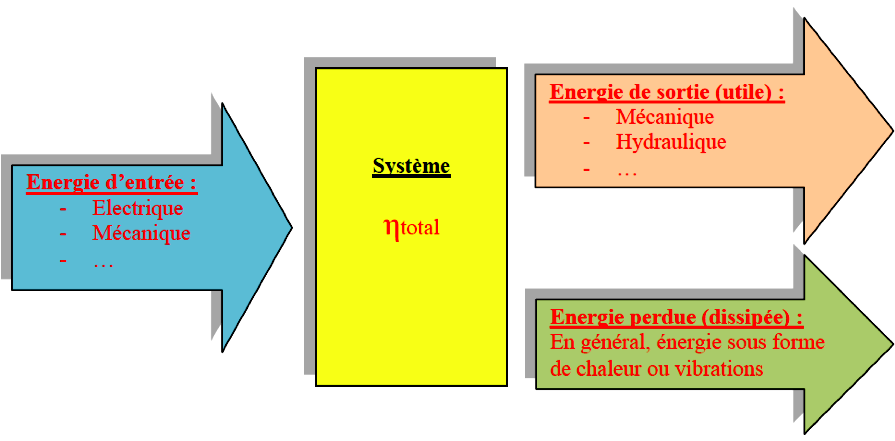
\includegraphics[width=0.8\textwidth]{images/rendement.png}
\end{center}

\subsection{Rendement d'un système décomposable}
Dans le cas d'un système décomposé en sous-systèmes, le rendement total correspond au produit des rendements de chacun des sous-systèmes : 
\begin{center}
    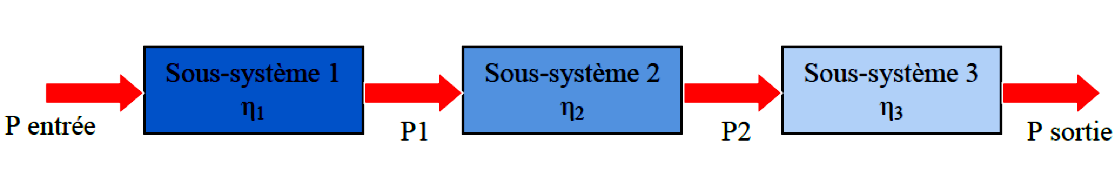
\includegraphics[width=0.8\textwidth]{images/rendement_multiple.png}
\end{center}

\begin{exemple}
    $$\eta_{\text{global}} = \frac{P_{\text{sortie}}}{P_{\text{entrée}}} = \frac{P_{\text{sortie}}}{P_{\text{2}}} \frac{P_{\text{2}}}{P_{\text{1}}} \frac{P_{\text{1}}}{P_{\text{entrée}}} = \eta_3 \times \eta_2 \times \eta_1$$
\end{exemple}
    \begin{defi}
     Dans le cas général d'un systèmes divisé en $n$ sous-systèmes :  
       $$ \eta_{\text{global}} = \eta_1 \times \eta_2 \times \dots \eta_n $$
    \end{defi}

\subsection{Ordre de grandeur de quelques rendements}
\subsubsection{Moteur thermique (à explosion) :}
\begin{center}
    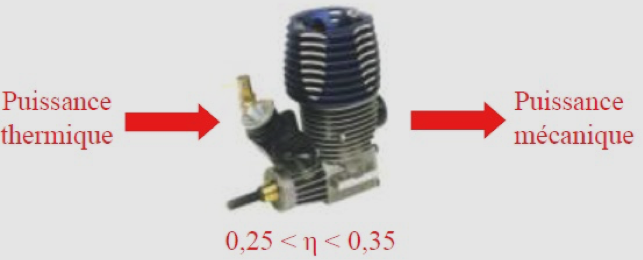
\includegraphics[width=0.5\textwidth]{images/thermique.png}
\end{center}

\subsubsection{Moteur électrique :}
\begin{center}
    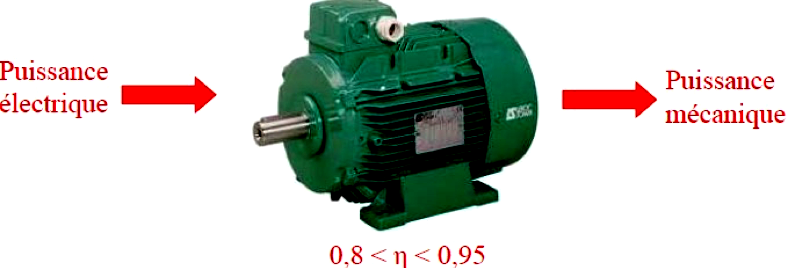
\includegraphics[width=0.5\textwidth]{images/eletrique.png}
\end{center}

\subsubsection{Roulement à billes :}
\begin{center}
    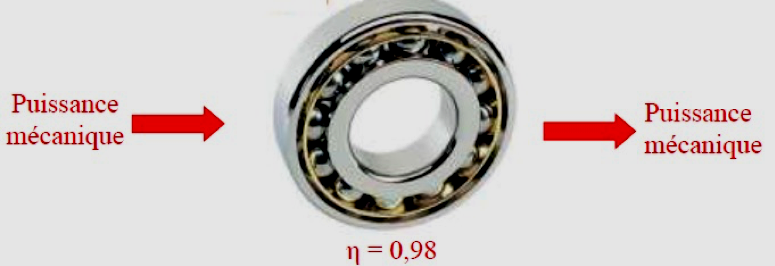
\includegraphics[width=0.5\textwidth]{images/roulement.png}
\end{center}

\subsubsection{Engrenages à denture droite :}
\begin{center}
    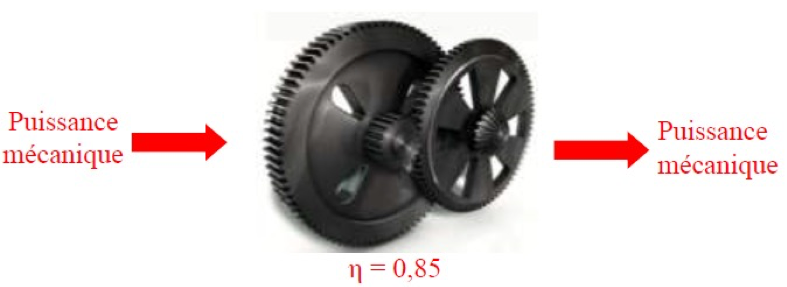
\includegraphics[width=0.5\textwidth]{images/engrenage.png}
\end{center}




\end{document}
